\section{Introduction}
\label{Introduction}

Processor and memory technologies have been developed with different
goals in mind. While processor scaling has focused on speed
improvements, memory scaling has primarily focused on increasing
capacity. The difference in each technology's scaling has led to the
Memory Wall~\cite{MemWall} -- the increasing gap between processor and
memory performance. Data prefetching is one important technique that
has been developed to minimize the effects of this trend.

\begin{figure}[t]
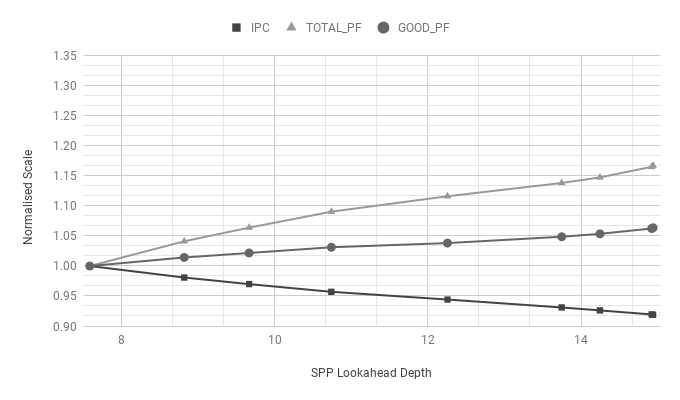
\includegraphics[width=0.95\columnwidth]{Motivation}
\caption{The impact of aggressive prefetching on performance for {\tt 603.bwaves\_s}. 
The number of useful prefetches increases with aggressiveness
slower than total prefetches, which wastes bandwidth and 
harms performance.}
\label{Fig:Motivation}
\end{figure}

An ideal prefetching scheme would perfectly capture a program's memory
access pattern, and then predict and pre-load the needed data into the
processor's caches in a timely manner.  Memory access patterns may be
simple, such as accessing every item in an array with a for-loop, or
very complex, such as chasing pointers through dynamically-allocated
memory. All prefetchers are designed around a fundamental trade-off between
two important metrics: coverage and accuracy. Prefetcher coverage
refers to the fraction of baseline cache misses that the prefetcher
pulls into the cache prior to their reference.  For example, if an
application experiences 1,000 cache misses without a prefetcher, while
800 of those cache misses become hits with a prefetcher, then the
prefetcher has 80\% coverage for that application.  Prefetcher
accuracy refers to the fraction of prefetched cache lines that end up
being used by the application. So if a prefetcher prefetches 1,200
cache lines, but only 800 of them are used by the application, then
that prefetcher's accuracy is 66.7\%.

Coverage and accuracy are generally at odds with one another, and as
one metric improves, the other usually gets worse. For example, when
an application accesses a new region of memory for the first time, a
na\"ive prefetcher may predict that all data in that region will be
used by the application.  This will clearly result in 100\% coverage
for that region, but with possibly a very low accuracy.  In fact, so
much cache capacity and bandwidth may be wasted prefetching unused
data that performance can ultimately be harmed by this strategy. At
the other extreme, another prefetcher may be overly conservative and
never prefetch anything, wasting no capacity or bandwidth, and
achieving 0\% prefetch coverage.

Figure~\ref{Fig:Motivation} illustrates the above scenario.  Here we
consider a state-of-the-art lookahead prefetcher -- SPP~\cite{SPP}.
Lookahead prefetchers such as SPP provide a mechanism to speculate an
arbitrary number of references ahead of the initial triggering access.
In SPP, a throttling confidence threshold is then used to ensure that
the lookahead stops when confidence falls too low to ensure that
prefetches are accurate.  In the figure, we iteratively re-tuned 
this threshold to allow the prefetcher to lookahead a fixed
depth from 7 to 15. The figure depicts the behavior 
of the {\tt 603.bwaves\_s} SPEC CPU 2017 benchmark. The IPC, the 
total number of prefetches issued by the prefetcher (TOTAL\_PF), 
and the actual useful predictions (GOOD\_PF), all have been normalized 
to lookahead depth 7. As the lookahead
depth increases, so do useful prefetches, and hence coverage. This
coverage, however, comes at the cost of total prefetches increasing at
an even higher rate. This leads to cache pollution and bandwidth
contention, and leads to a reduction in IPC.  

Therefore, a delicate balance between coverage and accuracy is
required for a prefetcher to maximize its performance impact.
Prefetchers are generally designed with internal mechanisms to monitor
their accuracy, and throttling mechanisms that can be tuned for either
coverage or accuracy.  The more irregular an application's memory
access pattern is, the more difficult it is to accurately predict
every access, so a prefetcher will have to be tuned more toward
coverage (and away from accuracy) in order to gain any benefit. This
may be especially dangerous to do in the context of a multi-core
processor, where overly aggressive prefetching in one core can waste
shared resources, such as last-level cache (LLC) capacity, and
off-chip bandwidth, impacting the performance of other
cores~\cite{Friendly}.


Here, we propose Perceptron-based Prefetch Filtering (PPF) as an
enhancement to existing state-of-the-art prefetchers, allowing them to
speculate deeply to achieve high coverage while filtering out the
inaccurate prefetches this deep speculation implies.  PPF works by
observing the stream of candidate prefetches generated by a
prefetcher, and then rejects those that are predicted by the
online-trained neural model to be inaccurate.  The state-of-the-art
prefetcher that we use to evaluate PPF in this paper is the Signature
Path Prefetcher (SPP)~\cite{SPP}, however as we describe, PPF can be
designed to benefit any prefetcher.  In this design, PPF replaces
SPP's existing confidence-based throttling mechanism, which itself was
a highly tuned feature of that prefetcher.  Because PPF is so much
more effective at rejecting inaccurate prefetches than SPP's 
{internal} mechanism, we are free to re-tune the rest of 
SPP's design around maximizing coverage. The result is an increase 
in both accuracy and coverage, and a notable increase in performance.


This paper describes PPF, explains its merits, offers analysis, and
outlines the scope for future research. Its contributions are:

\begin{itemize}

\item An on-line neural model used for hardware data prefetching.
  Previous work in this area either relied on program
  semantics~\cite{Semantics} or were application
  specific~\cite{Datacenter}.

\item Implementing PPF filtering a state-of-the-art prefetcher, giving
  a significant performance improvement compared to previous work. PPF
  learns to adapt itself to shared resource constraints, leading to
  further increased performance in multi-core and
  bandwidth-constrained environments.

\item A methodology for determining an appropriate set of features for
  prediction, regardless of the underlying prefetcher used.  More
  details are explained in Section \ref{Method-Features}.

\end{itemize}

In a single core configuration, PPF increases performance by 3.78\%
compared to the underlying prefetcher, SPP. In a multi-core system running a
mixes of memory intensive SPEC CPU 2017 traces, PPF saw an improvement
of 11.4\% over SPP for a 4-core system, and 9.65\% for an 8-core system.
